\subsection{连续映射的典范分解}

设 X 与 Y 是两个拓扑空间，\(f: X \rightarrow Y\) 是一个连续映射，R 是 X 上的等价关系 \(f(x) = f(y)\)。考虑典范分解

\[
f: \mathrm{X} \xrightarrow {\varphi} \mathrm{X} / \mathrm{R} \xrightarrow {g} f (\mathrm{X}) \xrightarrow {\psi} \mathrm{Y}
\]

其中 \(\varphi\) 是 X 到商空间 X/R 上的典范（满）映射，\(\psi\) 是子空间 \(f(X)\) 到 Y 中的典范单射，而 \(g\) 是与 \(f\) 相伴的双射（《集合论》R，§ 5，第 3 目）。立即可见 \(g\) 是连续的（由第 4 目命题 6）；它也是关于商结构的一个一般结果的特例。（参见《集合论》第四章，§ 2，第 6 目。）但双射 \(g\) 未必是同胚。

\pandocbounded{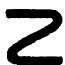
\includegraphics[keepaspectratio]{images/part001_a90573a3.jpg}}

命题 8. 设 \(f = \psi \circ g \circ \varphi\) 是连续映射 \(f: X \to Y\) 的典范分解，且设 \(R\) 表示等价关系

\[
f (x) = f (y).
\]

则下列三个条件等价：

\begin{enumerate}
\def\labelenumi{\alph{enumi})}
\item
  \(g\) 是由 \(\mathbf{X} / \mathbf{R}\) 到 \(f(\mathbf{X})\) 上的一个同胚。
\item
  在 \(f\) 之下，每个关于 \(\mathbf{R}\) 饱和的开集的像是子空间 \(f(\mathbf{X})\) 中的一个开集。
\item
  在 \(f\) 之下，每个关于 \(\mathbf{R}\) 饱和的闭集的像是子空间 \(f(\mathbf{X})\) 中的一个闭集。
\end{enumerate}

因为条件 b){[}resp. c){]}表达的是：X/R 中每个开（相应地，闭）集在 g 下的像是 \(f(\mathbf{X})\) 中的一个开（相应地，闭）集。

例。设 X 是拓扑空间，\((\mathbf{X}_{i})_{i\in I}\) 是 X 的一个覆盖，Y 是 X 的诸子空间 \(X_{v}\) 的和；则存在 Y 的一个分成既开又闭的子空间的分拆 \((\mathbf{Y}_{i})_{i\in I}\)，且对每个 \(i\in I\) 存在一个同胚 \(f_{i}:Y_{i}\to X_{i}\)。设 \(f:Y\to X\) 是与 \(f_{i}\)（在 \(Y_{i}\) 上，对每个 \(i\in I\)）相一致的连续映射，且设 R 是等价关系 \(f(x)=f(y)\)；于是商空间 Y/R 是把诸 \(Y_{i}\)"粘合"在一起得到的（§2，第 5 目）。考虑与 f 相伴的双射 \(g:Y/R\to X\)；一般说来 g 不是同胚，如下例所示：每个 \(X_{i}\) 都由单个点组成而 X 不是离散的。然而，若诸 \(X_{i}\) 的内部覆盖 X，或 \((\mathbf{X}_{i})\) 是 X 的一个局部有限闭覆盖，则 g 是同胚：因为若 U 是 Y 的任一关于 R 饱和的开子集，则对每个 \(i\in I\)，集合

\[
f (\mathbf {U}) \cap \mathbf {X} _ {i} = f _ {i} (\mathbf {U} \cap \mathbf {Y} _ {i})
\]

在 \(X_{i}\) 中是开集，且断言由第 1 目命题 3 得出。

下面的命题给出 \(g\) 是同胚的一个简单充分条件：

命题 9. 设 \(f: \mathbf{X} \to \mathbf{Y}\) 是一个连续满射，且设 \(\mathbf{R}\) 表示等价关系 \(f(x) = f(y)\)。若存在连续截面 \(s: \mathbf{Y} \to \mathbf{X}\)（与 \(f\) 相伴（《集合论》第二章，§ 3，第 8 目，定义 11）），则映射 \(g: \mathbf{X} / \mathbf{R} \to \mathbf{Y}\)（与 \(f\) 相伴）是一个同胚，且 \(s\) 是由 \(\mathbf{Y}\) 到子空间 \(s(\mathbf{Y})\)（\(\mathbf{X}\) 的子空间）上的一个同胚。

因为若 \(\varphi: \mathbf{X} \to \mathbf{X} / \mathbf{R}\) 是典范映射，则 \(g\) 与 \(\varphi \circ s\) 都是双射、连续且互逆；同样，\(s\) 与 \(f\) 在 \(s(\mathbf{Y})\) 上的限制都是双射、连续且互逆。

若 R 是拓扑空间 X 上的一个等价关系，且

\[
\varphi : \mathbf {X} \rightarrow \mathbf {X} / \mathbf {R}
\]

是典范映射，连续截面 \(s: \mathbf{X} / \mathbf{R} \to \mathbf{X}\)（与 \(\varphi\) 相伴）也称为 \(\mathbf{X}\) 关于 \(\mathbf{R}\) 的连续截面（参见《集合论》第二章，§ 6，第 2 目）；于是子空间 \(s(\mathbf{X} / \mathbf{R})\)（\(\mathbf{X}\) 的子空间）同胚于 \(\mathbf{X} / \mathbf{R}\)。若给定了 \(s(\mathbf{X} / \mathbf{R})\)，则 \(s\) 被唯一确定；\(s(\mathbf{X} / \mathbf{R})\) 常被（滥用语言地）称为 \(\mathbf{X}\) 关于 \(\mathbf{R}\) 的一个（连续）截面。

\pandocbounded{
\includegraphics[keepaspectratio]{images/part001_feb98675.jpg}}

拓扑空间关于一个等价关系的连续截面未必存在（习题 12）。

